\documentclass[titlepage]{article}

\usepackage[czech]{babel}
\usepackage{graphicx}
\usepackage{tikz}
\usepackage{hyperref}
\usepackage{dirtree}
\usepackage{amsmath}

\makeatletter
\tikzset{
    database/.style={
        path picture={
            \draw (0, 1.5*\database@segmentheight) circle [x radius=\database@radius,y radius=\database@aspectratio*\database@radius];
            \draw (-\database@radius, 0.5*\database@segmentheight) arc [start angle=180,end angle=360,x radius=\database@radius, y radius=\database@aspectratio*\database@radius];
            \draw (-\database@radius,-0.5*\database@segmentheight) arc [start angle=180,end angle=360,x radius=\database@radius, y radius=\database@aspectratio*\database@radius];
            \draw (-\database@radius,1.5*\database@segmentheight) -- ++(0,-3*\database@segmentheight) arc [start angle=180,end angle=360,x radius=\database@radius, y radius=\database@aspectratio*\database@radius] -- ++(0,3*\database@segmentheight);
        },
        minimum width=2*\database@radius + \pgflinewidth,
        minimum height=3*\database@segmentheight + 2*\database@aspectratio*\database@radius + \pgflinewidth,
    },
    database segment height/.store in=\database@segmentheight,
    database radius/.store in=\database@radius,
    database aspect ratio/.store in=\database@aspectratio,
    database segment height=0.1cm,
    database radius=0.25cm,
    database aspect ratio=0.35,
}
\makeatother



\title{Generátor úloh do aplikované kryptografie\\Kontrolní studie}
\author{Michal Homola,\\Dominik Chrenčík,\\Jiří Marák,\\Vojtěch Lukáš}

\begin{document}
\maketitle

\tableofcontents

\section*{Úvod}
%TODO: Úvod, o projektu, autoři, kdo má co na práci apod.

\section{Architektura}
Schéma připravovaného systému lze vidět na obr.\,\ref{fig:sys}. Úlohy budou uloženy v SQL databázi. K~této databázi bude mít přístup pouze webový PHP~server. Ten slouží jako \uv{prostředník} mezi klientem a databází. Dále by měl do úloh vkládat náhodná data (klíče apod.) a~případně také vyhodnocovat výsledky. 
Klientská aplikace bude fungovat jako přístupový bod a sehrávat roli prezentační vrstvy. Pro jednoduchost bude vyvinuta v jazyce Python s oddělenou logickou vrstvou. Bude tedy možné na tuto vrstvu napojit i jednoduché grafické rozhraní. 
\begin{figure}[h!]
    \centering
    

\begin{tikzpicture}
    \draw (-.5,0) node[database, label=below: SQL databáze, database radius = .5cm, database segment height = .25cm]{};
    \draw[densely dotted, thick] (0,0) -- (1.5,0);
    \draw (1.5, -.7) rectangle (2.5, .7);
    \draw (1.5, .35) -- (2.5, .35);
    \draw (1.5, 0) -- (2.5, 0);
    \draw (1.5, -.35) -- (2.5, -.35);
    \draw (2, -.7) node[below]{.NET server};

    \draw[dashed] (-2,-1.5) rectangle (3.5,1.5) coordinate (box_right);
    \draw (.75, 1.5) node[above]{Microsoft Azure};
    \draw[dashed] (box_right) ++(down: 1.5) -- ++(right: 2) coordinate (pc_left); 
    \draw (pc_left) rectangle ++(1, .75);
    \draw (pc_left) -- ++(-.25, -.25) -- ++(right: .75) coordinate (pc_text) -- ++(right: .25) -- ++(.25, .25);
    \draw (pc_text) node[below]{Python klient};

\end{tikzpicture}    
    \caption{Schéma systému}
    \label{fig:sys}
\end{figure}




\subsection{Databáze úloh}\label{sec:databaze_uloh}

V rámci návrhu kryptografických úloh, byly úlohy co nejvíce standardizované, z důvodu jejich uložení v jednotné databázi. Zároveň musí být výsledky jednoznačné tak, aby byly dobře porovnatelné s výsledky zadanými řešitelem. Proto jsou výsledky koncipovány jako číslo, či prosté \uv{ano/ne}.      

 V databázi jsou zahrnuty různé typy kryptografických úloh, aby bylo možné si vyzkoušet různé druhy kryptografických algoritmů a technologií. Součástí každé úlohy bude i nápověda k řešení, tak aby i řešitel, který si neví rady, mohl příklad vyřešit.

\subsubsection{Konstrukce databáze}
V tabulce \ref{tab:struktura_databaze} lze vidět současnou strukturu SQL databáze. Sloupec \textbf{ID} slouží jako primární klíč databáze, v buňce \textbf{Zadání} se pak nachází textový popis úlohy. Zde stojí za povšimnutí, že všechny číselné hodnoty důležité k výpočtu jsou nahrazeny zástupnými znaky $\$n$. Na místa těchto znaků bude logika v back-endu vkládat vygenerované hodnoty. Díky tomu bude možno jednu úlohu řešit vícekrát, pokaždé s jinými parametry. \textbf{Kód} úlohy pak slouží pro snazší rozlišení úloh. Uživatel si bude moct vybrat jaký typ bude chtít řešit, back-end si tuto úlohu vytáhne z databáze, opatří ji vygenerovanými operandy a spolu se správným výsledkem a nápovědou z buňky \textbf{Nápověda} ji zašle uživateli.  
 \begin{table}
    \centering
    \caption{Struktura SQL databáze}
    \label{tab:struktura_databaze}
    \vspace{.5em}
    \begin{tabular}[h]{| l | p{6cm} | l | l |}
        \hline
        \textbf{ID} & \textbf{Zadání} & \textbf{Kód} & \textbf{Nápověda} \\
        \texttt{INT} & \texttt{TEXT} & \texttt{VARCHAR(5)} & \texttt{TEXT} \\
        \hline\hline
        1 & Rozhodněte (ano/ne) zda je číslo $n=\$1$ prvočíslo & \texttt{PR} & \dots \\
        \hline
        2 & Zašifrujte zprávu $m=\$4$, pomocí RSA kryptosystému. Prvočísla jsou $p=\$1;\ q=\$2$, a soukromý klíč je $e=\$3$ & \texttt{RSAe} & \dots\\
        \hline
        \vdots & \vdots & \vdots & \vdots \\
        \hline
    \end{tabular}
 \end{table}
    

\subsection{Typy úloh}
\subsubsection{RSA}
Část  úloh zahrnuje výpočet RSA algoritmu. Zadáno je zde šifrování nebo naopak dešifrování zprávy pomocí zadaného klíče algoritmem RSA.

Vygenerování klíče: 
\begin{align*}
     n &= p \cdot q \\
    \phi(n) &= (p-1) \cdot (q-1) \\
    e, d &= \text{pro které platí}\ (d \cdot e) \bmod \phi(n) = 1 \\
    \text{Veřejný klíč: } (n, e) \\
    \text{Soukromý klíč: } d
\end{align*}

Šifrování:
\begin{align*}
    \text{Zpráva } M \\
    C &= M^e \bmod n
\end{align*}

Dešifrování:
\begin{align*}
    \text{Kryptogram: } C \\
    M &= C^d \bmod n
\end{align*}


\subsubsection{Diffie-Hellman}
Další úloha je použití protokolu Diffie-Hellman, který slouží k výměně klíčů mezi dvěma stranami bez potřeby sdílení klíčů předem. Protokol je založen na principech asymetrické kryptografie a umožňuje ustanovení šifrovacího klíče přes nedůvěryhodné médium.
V úloze se ověřuje pochopení procesu výměny a výpočtu klíčů mezi dvěma stranami.
\begin{figure}[h]
\centering
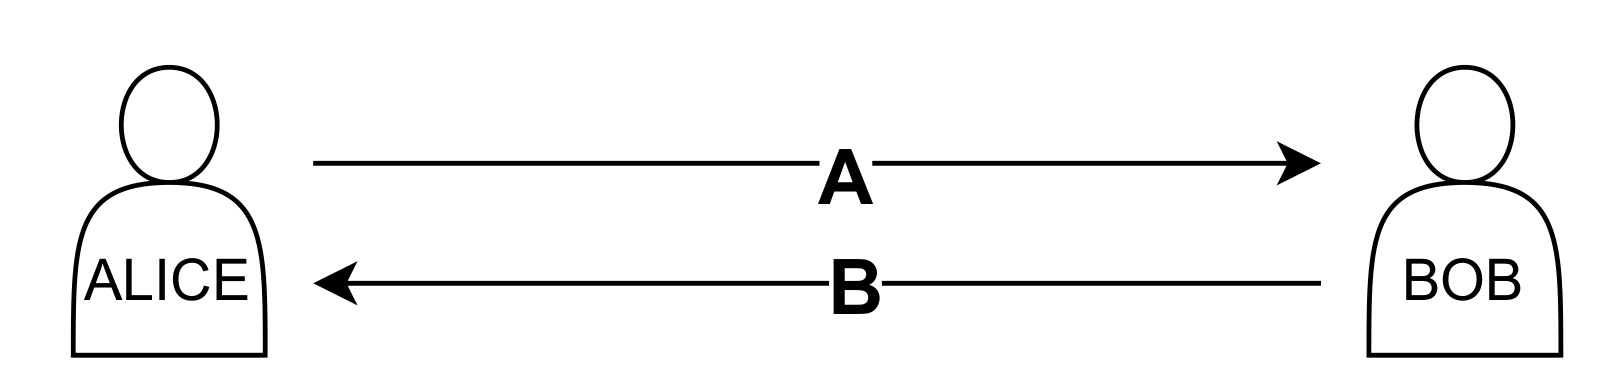
\includegraphics[width=0.7\textwidth]{dh.png}
\caption{\label{fig:DH}Diffie-Hellman - předání klíčů}
\end{figure}




\begin{center}
\renewcommand{\arraystretch}{1.5}
\begin{tabular}{|c@{\hspace{5mm}}|c|}
    \hline
  ALICE & BOB \\
  \hline
  $a\in_{R} Z_{q} $ & $b\in_{R} Z_{q} $\\
  \hline
  $A=g^{a}mod\,p$& $B=g^{b}mod\,p$\\
  \hline
  $K=B^{a}mod\,p$ &  $K=A^{b}mod\,p$ \\
  \hline
\end{tabular}
\end{center}




\subsubsection{Test prvočíselnosti}
Test prvočíselnosti se také nachází v databázi úloh. Tato úloha zahrnuje ověření, zda je zadané číslo prvočíslo či nikoliv, což je základem pro mnoho kryptografických algoritmů. Pro testovaní zda je číslo prvočíslem lze použít například Lucas–Lehmerův test prvočíselnosti pro Mersennova prvočísla:
\begin{align*}
    &\text{Nechť } p \text{ je liché prvočíslo a } M = 2^p-1 \\
    &\text{Nastavíme } s_0 = 4 \\
    &\text{Pro } i=1,2,\dots,p-2: \\
    &\quad s_i = (s_{i-1}^2-2) \bmod M \\
    &\text{Pokud } s_{p-2} = 0 \text{, pak } M \text{ je Mersennovo prvočíslo.} \\
    &\text{Jinak } M \text{ je složené číslo.}
\end{align*}

\subsubsection{GCD a LCM}
Dále jsou zde také příklady na výpočet nejmenšího společného ná\-so\-bku (Le\-ast Com\-mon Multiple -- LCM) 
a největšího společného dělitele (GCD -- Greatest common divisor). 
které také najdou uplatnění v kryptografii. Při řešení těchto příkladů lze využít například rozklad na prvočísla.
\newline

\subsubsection{Modulární aritmetika}
V databázi jsou také příklady na modulární aritmetiku, jako výpočet operace modulo nebo kongruence. 
Operace modulo $(mod\,n)$ vrátí pouze zbytek vstupního čísla po
dělení číslem $n$.


Cele číslo je kongruentní modulo $n$ s celým číslem $b$ tehdy, když
je rozdíl $a - b$ dělitelný číslem $n$. Zapisujeme jako $a \equiv b \pmod n$.
Pro kongruence modulo platí:
\begin{align*}
    a \equiv b \pmod{m} \\
    b \equiv a \pmod{m} \\
    % a  neco 
\end{align*}

%% next section?
V dalším vývoji by mohla být nápověda rozdělena na více úrovní, tak aby si je řešitel mohl postupně vyžádat v případě, že mu bude postačovat pouze malá nápověda a potřebuje pouze \uv{nakopnout}, nebo si neví rady a potřebuje nápovědu větší. Taktéž budu přidány další úlohy z oblasti aplikované kryptografie.   

\subsection{Back-end}
Architektura back-endu je navržena podle doporučení REST API. Původní návrhy řešení počítaly s využitím .NET serveru na portálu Microsoft Azure. Nakonec bylo ale upřednostněno řešení využívající PHP server. Celé řešení back-endu je založeno na \cite{restapi}. Od začátku byl projekt vyvíjen přímo na serveru pro usnadnění přístupu. 

\subsection{Výpočet řešení úloh}

\subsubsection{API dotazy}\label{sec:api_dotazy}
\begin{table}[b]
    \centering
    \caption{Tabulka API dotazů}
    \label{tab:api_dotazy}
    \vspace{.5em}
    \begin{tabular}{|l | p{5cm} |}
        \hline
        \textbf{URL} & \textbf{Popis} \\
        \hline \hline
      \texttt{/index.php/alltasks} & Vrátí JSON objekt obsahující všechny úlohy z databáze \\
        \hline
        \texttt{/index.php/task?code=<kód>} & Vrátí jednu (nebo více) úloh(u) daného typu \\
        \hline
        \texttt{/index.php/randomtask} & Vrátí jednu náhodně vybranou úlohu \\
        \hline
    \end{tabular}
\end{table}

V rámci projektu jsou využity dotazy z tabulky \ref{tab:api_dotazy}. Struktura těchto dotazů respektuje doporučení REST API. 

\subsubsection{Generování hodnot}\label{sec:generovani_hodnot}
Úkolem back-end serveru bude také generování a vkládání hodnot do textu úlohy. Toto bude mít na starosti samostatný modul, který podle kódu vyžádané úlohy vygeneruje potřebné hodnoty, vloží je na místo tokenů \uv{$\$n$} (viz tabulka~\ref{tab:struktura_databaze}). Takto připravená data již může převzít další modul a odeslat je uživateli. 

Neméně důležitým úkolem této sekce je také výpočet správného výsledku pro vyhodnocení. Správný algoritmus pro výpočet bude zvolen podle kódu úlohy. Vypočtená hodnota bude opět předána dalšímu modulu, který je bude odesílat uživateli. 

\subsubsection{Obsah JSON odpovědi}\label{sec:obsa_json}
Jak již bylo zmíněno v předchozích odstavcích, JSON odpovědi budou obsahovat kromě buněk z SQL databáze také další hodnoty vygenerované serverem. V tuto chvíli vypadá návrh JSON objektu následovně:
\begin{itemize}
    \item název úkolu,
    \item zadání úkolu,
    \item kód úkolu,
    \item nápověda,
    \item správné řešení.
\end{itemize}


\subsection{Front-end}
Tato část projektu bude mít formu jednoduché aplikace vyvinuté v jazyce Python. Nejprve si vyžádá seznam úloh, které jsou uživateli k dispozici. Uživatel si z výběru zvolí jednu úlohu, ta je mu pak prezentována. V tuto chvíli má uživatel také možnost vyžádat si nápovědu. Po zadání řešení je pak vyhodnocena správnost výsledku. Nyní se nabízí možnost počítat skóre a čas potřebný k vyřešení. 

Aplikace může mít více podob. Implicitně se počítá s konzolovou aplikací, ale nic nebrání ani vývoji elementárního grafického rozhraní pro příjemnější uživatelský zážitek. 



\section{Současný stav}
Tým využívá dva GIT repozitáře. K nahlédnutí jsou \href{https://github.com/voytex/kry_gen}{zde} a \href{https://github.com/voytex/kry_gen-backend}{zde}.
\subsection{Databáze úloh}
V čase odevzdání této studie je navrhnuto 7 různých kryptografických úloh v souladu s jejich návrhem v sekci \ref{sec:databaze_uloh}. Všechny tyto úlohy jsou opatřeny tokeny \uv{$\$n$} a nápovědami. Jsou také již nahrané v SQL databázi na serveru. 
\subsection{Back-end}
Webová služba je v tuto chvíli zčásti hotová a publikovaná na adrese \url{http://vut-fekt-mpckry-gr14.8u.cz/index.php}. Implementováno jsou nyní reakce na API dotazy (viz sekce \ref{sec:api_dotazy} a \ref{sec:obsa_json}), chybí implementovat generování hodnot (viz sekce \ref{sec:generovani_hodnot}). V textu JSON odpovědí jsou tokeny \uv{$\$n$} nyní ještě nenahrazeny. Odpověď nyní také ještě neobsahuje hodnotu se správným výsledkem. 



Funkčnost lze ukázat na následujícím odkazu, který respektuje API popsané v tabulce \ref{tab:api_dotazy}:
\url{http://vut-fekt-mpckry-gr14.8u.cz/index.php/task?code=dh}.
Po kliknutí na odkaz by se měl uživateli zobrazit v prohlížeči JSON objekt obsahující úlohu týkající se DH protokolu. 

\subsection{Front-end}
Této části systému bylo prozatím věnováno nejméně pozornosti. Byl vyvinut ukázkový skript, který dokazuje úspěšné propojení s webovou službou, zobrazení všech úloh, žádost a přijetí jedné konkrétní úlohy a výpis nápovědy. To vše lze vidět na obr.\,\ref{fig:front_end}

\begin{figure}
    \centering
    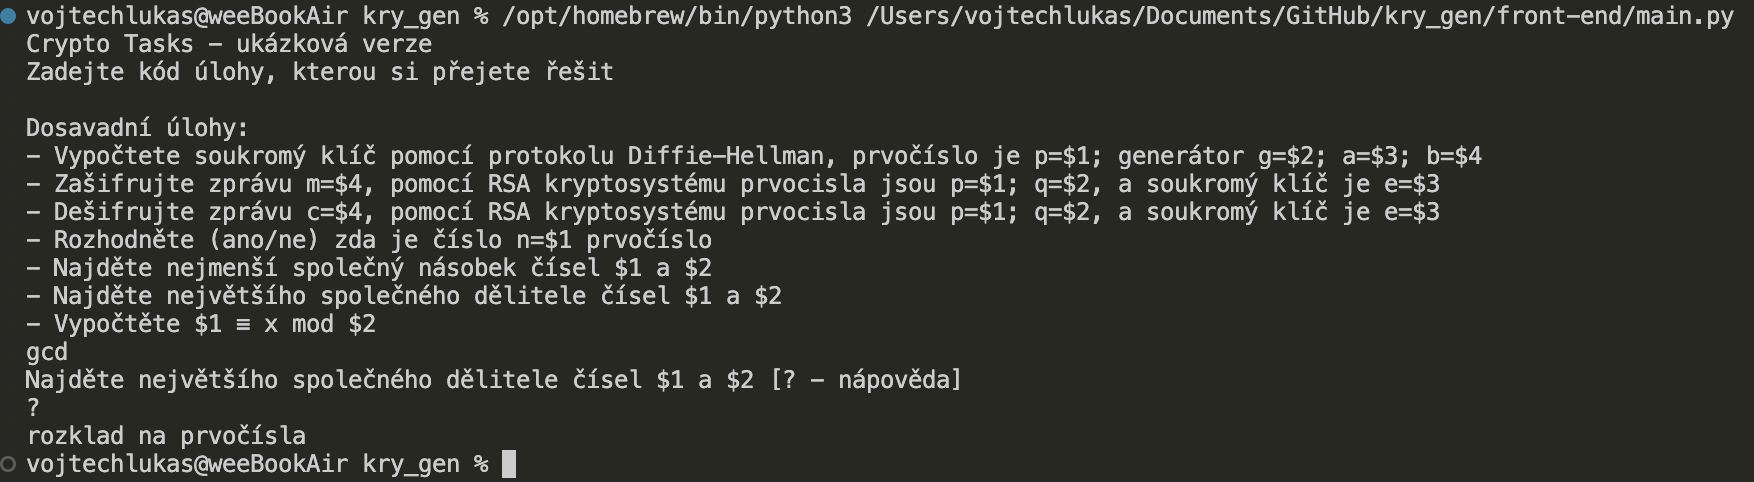
\includegraphics[width=.8\linewidth]{frontend.png}
    \caption{Ukázkový průchod front-end skriptem}
    \label{fig:front_end}
\end{figure}
% \subsubsection{Soubory webového serveru}
% \dirtree{%
%     .1 web.
%     .2 Model.
%     .3 Database.php.
%     .3 TaskModel.php.
%     .2 Controller.
%     .3 Api.
%     .4 BaseController.php.
%     .4 TaskController.php.
%     .2 inc.
%     .3 config.php.
%     .3 bootstrap.php.
%     .2 index.php.
% }
% \vspace{1em}
% Moduly ve složce \texttt{Model} slouží k propojení a komunikaci s databází. Modul \texttt{Task\-Controller.php} je využit ke zpracování různých požadavků z uživatelské aplikace. Soubory ve složce \texttt{inc} by se daly označit jako \uv{servisní moduly}: \texttt{config.php} definuje přístupové údaje k databázi jako konstanty\footnote{Vzhledem k citlivé povaze obsažených informací je tento soubor vyřazen z verzování pomocí záznamu v \texttt{.gitignore}.}; modul \texttt{boot\-strap.php} pak obstarává správné propojení modulů. Modul \texttt{index.php} je pak ten, který přímo komunikuje s klientskou aplikací, třídí její požadavky a korektně na ně odpovídá. 

\section{Členové týmu}
\subsection*{Michal Homola}
Má na starosti vývoj logiky generování hodnot a výpočtu správného výsledku.
\subsection*{Dominik Chrenčík}
Vyvíjí front-end aplikace.
\subsection*{Jiří Marák}
Vymýšlí kryptografické úlohy a nápovědy k nim.
\subsection*{Vojtěch Lukáš}
Má na starosti back-end a API. 

\section*{Závěr}



\begin{thebibliography}{9}
    \bibitem{restapi}
    SONI, Sajal. How to build a simple REST API in PHP. \emph{En\-va\-to Tuts+} [on\-li\-ne]. 27-5-2021 [cit. 2023-03-25]. Dostupné z: \url{https://code.tutsplus.com/tutorials/how-to-build-a-simple-rest-api-in-php--cms-37000}
\end{thebibliography}

\end{document}